
%********** Chapter 7 **********
\chapter{Linked Robots}\index{linked list}\index{projects!Linked Robots}

\section{Introduction}

This chapter introduces the final project, Linked Robots.  The program creates a dynamic data structure (a linked list) of robot objects and demonstrates a few of the capabilities of linked lists.  In particular, the ability to modify the length of the linked list, by adding and deleting data elements from it, while the program is running.  The program doesn't do very much, but it introduces the possibilities inherent in dynamic data structures and is the basis for more complex two dimensional simulations.  For example, it could be combined with the Robot World program to allow multiple robots per cell or with the Electronic Pet to allow a user to easily play with multiple pets at the same time.

This project reviews the topics from the earlier chapters, particularly classes and pointers, and introduces three new topics:
\begin{tight_itemize}
\item Dynamic data structures
  \item Linked lists
   \item Recursion
\end{tight_itemize}

A linked list is a a dynamic data structure that allows a program to create and delete an unlimited number of data elements dynamically.  Recursion is a powerful programming technique in which a function calls itself or two (or more) functions call each other.

\section{The Program}

The Linked List program requires three new files: 
the main file (Listing~\ref{listing:robotlinkedlist}), which can have any name, and two library files: ``node.h'' (consisting of  Listing~\ref{listing:nodeh} followed by
Listing~\ref{listing:nodecpp}) and ``linkedlist.h'' (consisting of 
Listing~\ref{listing:llh} followed by
Listing~\ref{listing:llcpp}).  Note that the names of the library files are used in \cf{include} statements in the other files, so can't be changed (unless the \cf{include} statements are also changed).  The file ``robot.h'' from the previous project should  also be available to the program.  As always, as the program is entered, try to figure out what the commands do.  Most of them should be very familiar by now, but some of the syntax (particularly in the code from Listing~\ref{listing:nodecpp} and Listing~\ref{listing:llcpp}) may be somewhat confusing.

\begin{minipage}{\textwidth}
\renewcommand*\thelstnumber{\the\value{lstnumber}}
\begin{lstlisting}[language=C++,numbers = left,xleftmargin=4.0ex, basicstyle=\small, emph={ll,num_robots,robot_ptr,i},emphstyle = \color{\mycolor},
showstringspaces=false,
caption = {Main program for the Linked Robots program.  The include statements (lines 4, 5, and 6) automatically include the code from the other listings.},
label={listing:robotlinkedlist}]
#include <iostream>
#include <cstdlib>
using namespace std;
#include"robot.h"
#include"node.h"
#include"linkedlist.h"
int main(){
   linkedlist ll;
   const int num_robots = 3;
   robot *robot_ptr;
   for(int i = 0; i < num_robots; i++){
        robot_ptr = new robot(i);
        ll.insert(robot_ptr);
  }
  ll.print();
  cout <<"Turn all robots left:" << endl;
  ll.turnLeft();
  robot_ptr = new robot(99);
  ll.insert(robot_ptr);
  ll.remove(2);
  ll.print();
  return 0;
}
\end{lstlisting}
\end{minipage}

%-------------------------------------  Linked list ----------------------------------------
\begin{minipage}{\textwidth}
\renewcommand*\thelstnumber{\the\value{lstnumber}a}
\begin{lstlisting}[language=C++,numbers = left,xleftmargin=4.0ex, basicstyle=\small, emph={count,head},emphstyle = \color{\mycolor},
showstringspaces=false,
caption = {The declaration of the \cf{linkedlist} class, which holds the ``head'' of the linked list.},
label={listing:llh}]
class linkedlist{
    private:
         int count;
         node *head;
    public:
         linkedlist();
         void insert(robot *);
         void print();
         void turnLeft();
         void remove(int);
};
\end{lstlisting}
\end{minipage}

\textbf{Important:} two minor changes will need to be made to the \codefont{robot} class defined in the file ``robot.h.''  First, the member function \codefont{turnLeft()} will need to be made \emph{public} (to do this, simply move the function prototype from the private to the public region of the class definition). Although it is not necessary at this point, for future changes, it may be helpful to also make \cf{turnRight()} and \cf{forward()} public as well.  Second, a new (in-line) member function will need to be added to the \cf{robot} class.  Simply add the line\\
\codefont{
int getID() \{return ID;\}\\
} 
to the public section of the \cf{robot} class.  This new function returns the ID number of a robot, and is necessary for finding a robot by its ID (so it can be removed from the linked list).

Once all of the files have been created, compile the program containing the code from Listing~\ref{listing:robotlinkedlist}.  As always, there may be some copying errors that need to be fixed.  Once the program compiles, run it and see what it does.  By carefully comparing the code to the output it should be possible to figure out much of how the linked list works.  When dealing with linked lists it is often useful to sketch what the program is doing, particularly how the list is being constructed (see Figure~\ref{fig:llillustration}).  Try doing this with the Linked Robot program as it runs.

\begin{minipage}{\textwidth}
\renewcommand*\thelstnumber{\the\value{lstnumber}b}
\begin{lstlisting}[language=C++,numbers = left,xleftmargin=4.0ex, basicstyle=\small, emph={count,head,n,temp},emphstyle = \color{\mycolor},
showstringspaces=false,
caption = {The definition of the \cf{linkedlist} class functions. },
label={listing:llcpp}]
linkedlist::linkedlist(){
    head = NULL;
    count = 0;
}
void linkedlist::insert(robot *rp){
    node *n;
    n = new node;
    n->set_data(rp);
    n->set_next(head);
    head = n;
    count++;
}
void linkedlist::remove(int n){
    if(head == NULL)
         return;
    if((head->get_data())->getID() == n){
         node *temp;
         temp = head;
         head = head->get_next();
         temp -> remove_data();
         delete temp;
         count--;
    }
    else{
         if(head->remove(n) == 1)
             count--;    
    }
}
void linkedlist::print(){
    cout << "There are " << count;
    cout << " robots in the list: \n";
    if(head != NULL)
          head->print();
}
void linkedlist::turnLeft(){
      if(head != NULL)
            head->turnLeft();
}
\end{lstlisting}
\end{minipage}

%--------------------------------------- Node -----------------------------------------------

\begin{minipage}{\textwidth}
\renewcommand*\thelstnumber{\the\value{lstnumber}c}
\begin{lstlisting}[language=C++,numbers = left,xleftmargin=4.0ex, basicstyle=\small, emph={next,data},emphstyle = \color{\mycolor},
showstringspaces=false,
caption = {The declaration of the \cf{node} class. },
label={listing:nodeh}]
class node{
    private:
         node *next;
         robot *data;
    public:
        node();
        void set_next(node *n) {next = n;}
        void set_data(robot *d) {data = d;}
        node *get_next() {return next;}
        robot *get_data() {return data;}
        void print();
        void turnLeft();
        int remove(int);
        void remove_data() {delete data;}
};
\end{lstlisting}
\end{minipage}

\subsection{Linked Lists}\index{linked list}

\begin{figure}
%\centerline{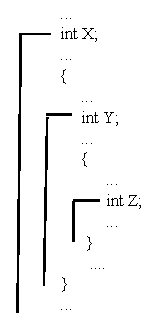
\includegraphics[width=9cm,height=6cm]{images/scope1.eps}}
\setlength{\unitlength}{1cm}
\begin{picture}(10,4)
\linethickness{0.3mm}


\put(0,3.6){\codefont{linked list object}}
\put(1.1,3.0){\codefont{head}}
\put(1.1,2.5){\codefont{count = 3}}

\color{\mycolor}{
\put(1,3.5){\line(1,0){2}}
\put(1,2.4){\line(1,0){2}}
\put(1,3.5){\line(0,-1){1.1}}
\put(3,3.5){\line(0,-1){1.1}}
\put(2.1,3.1){\vector(1,0){1.8}}

\put(4.1,3.5){\line(1,0){2}}
\put(4.1,2.4){\line(1,0){2}}
\put(4.1,3.5){\line(0,-1){1.1}}
\put(6.1,3.5){\line(0,-1){1.1}}
\put(5.1,3.1){\vector(1,0){1.7}}
\put(5.3,2.6){\vector(0,-1){1}}

\put(4.1,1.2){\line(1,0){2}}
\put(4.1,0.7){\line(1,0){2}}
\put(4.1,1.2){\line(0,-1){0.5}}
\put(6.1,1.2){\line(0,-1){0.5}}

\put(7.1,3.5){\line(1,0){2}}
\put(7.1,2.4){\line(1,0){2}}
\put(7.1,3.5){\line(0,-1){1.1}}
\put(9.1,3.5){\line(0,-1){1.1}}

\put(8.1,3.1){\vector(1,0){1.7}}
\put(8.3,2.6){\vector(0,-1){1}}

\put(7.1,1.2){\line(1,0){2}}
\put(7.1,0.7){\line(1,0){2}}
\put(7.1,1.2){\line(0,-1){0.5}}
\put(9.1,1.2){\line(0,-1){0.5}}

\put(10.1,3.5){\line(1,0){2}}
\put(10.1,2.4){\line(1,0){2}}
\put(10.1,3.5){\line(0,-1){1.1}}
\put(12.1,3.5){\line(0,-1){1.1}}
\put(11.1,3.1){\vector(1,0){1.7}}
\put(11.3,2.6){\vector(0,-1){1}}
\put(10.1,1.2){\line(1,0){2}}
\put(10.1,0.7){\line(1,0){2}}
\put(10.1,1.2){\line(0,-1){0.5}}
\put(12.1,1.2){\line(0,-1){0.5}}
}

\color{black}{
\put(4,3.6){\codefont{node object}}
\put(4.1,3.0){\codefont{next}}
\put(4.1,2.5){\codefont{data}}

\put(4,1.3){\codefont{robot object}}

\put(7,3.6){\codefont{node object}}
\put(7.1,3.0){\codefont{next}}
\put(7.1,2.5){\codefont{data}}

\put(7,1.3){\codefont{robot object}}

\put(10,3.6){\codefont{node object}}
\put(10.1,3.0){\codefont{next}}
\put(10.1,2.5){\codefont{data}}

\put(10,1.3){\codefont{robot object}}

\put(13,3.0){\codefont{NULL}}
}
\end{picture}
\caption{An illustration of a linked list.  The linked list consists of a series of \codefont{node} objects linked by pointers.  Each \codefont{node} object points to the next one in the list and to a \codefont{robot} object.  The head of the linked list is maintained by the \codefont{linked list} object, which also keeps track of the number of items in the list.  The last \cf{node} object points to \codefont{NULL}, thereby identifying the end of the linked list.  Other than the initial \codefont{linked list} object, the objects in a linked list  are usually nameless objects created with the \codefont{new} operator.  Objects can be added to or removed from the list simply by rearranging the \codefont{next} pointers.}
\label{fig:llillustration}
\end{figure}

A linked list is a \emph{dynamic} data structure.  A dynamic data structure is one in which the size of the data structure changes dynamically -- while the program is running.  In contrast an array is a \emph{static} data structure, once the size of the array is declared it cannot change size.\footnote{Part of an array could be empty, but the memory for the full array is still reserved in memory and an array can't be made larger.}  A linked list consists of a series of individual data structures ``linked'' together by pointers.  
In this program, the linked list consists of a series of \codefont{node} objects.  Each node object has a pointer called \codefont{next}, which points to the next node in the list, and a pointer called \codefont{data}, which points to the \codefont{robot} object associated with that node.  Figure~\ref{fig:llillustration} illustrates this idea.  In this example the beginning of the linked list is maintained by a separate \codefont{linked list} object.

\begin{minipage}{\textwidth}
\renewcommand*\thelstnumber{\the\value{lstnumber}d}
\begin{lstlisting}[language=C++,numbers = left,xleftmargin=4.0ex, basicstyle=\small, emph={next,data,temp},emphstyle = \color{\mycolor},
showstringspaces=false,
caption = {The definitions of the \cf{node} class functions. },
label={listing:nodecpp}]
node::node(){  // constructor
        next = NULL;
        data = NULL;
}
void node::print(){
        data->print();
        cout << endl;
        if(next != NULL)
              next -> print();
}
void node::turnLeft(){
        data -> turnLeft();
        if(next != NULL)
              next -> turnLeft();
        data -> print();
        cout << endl;
}
int node::remove(int n){
       if(next != NULL){
             if((next -> data) -> getID() == n){ // found the right ID
                  node *temp;
                  temp = next;
                  next = next -> next;
                  temp -> remove_data();
                  delete temp;
                  return(1);  // successfully removed
             }
            else{
                  return(next -> remove(n));  // try the next node
             }
     }
     return 0;     // given robot was never found
}
\end{lstlisting}
\end{minipage}  


Although linked lists and arrays both store a list of data elements, linked lists have several advantages over arrays.  First, because list items are created by \cf{new} and removed via \cf{delete}, the length of a linked list does not have to be determined in advance; it can change as needed as the program runs.  In addition, items can easily be added to, or removed from, the middle of a linked list by redirecting the pointers to include, or skip over, a node.  With an array, adding or removing an element from the middle of the array requires shifting all of the elements below the changed element.

Linked lists have two notable disadvantages.  First, the code for creating and manipulating a linked list is  more complicated than for an array.  However, a well-written linked list class encapsulates the complex parts of the code, making it easy to incorporate a linked list in other programs.  Second, linked lists don't allow for \emph{random access}\index{random access} the way that arrays do.  Accessing element $N$ of an array is a simple and quick operation.  Accessing element $N$ of a linked list requires ``stepping'' through the list until the $N$th element is found.\footnote{Basic linked lists require stepping through the list to find a particular element of the list.  However, more complex data structures can be created that, for example, combine a linked list with an array of pointers that point to various elements within the list.  This makes it possible to jump to a midpoint in the list.  But such hybrid structures are beyond the scope of this text.} 



\subsection{Recursion}\index{recursion}

A \emph{recursive} function is one that calls itself.\footnote{More generally, a program can have mutually recursive functions that call each other.}  To avoid infinite loops, a recursive function must have a \emph{terminating condition} that keeps the function from calling itself under some conditions.

Recursive functions are a natural method to step through dynamic data structures (like linked lists) or for programming recursively defined mathematical functions.  For example, the Fibonacci numbers can be defined by a function $f()$:\\
$\hspace*{1cm}f(0) = 0\\
\hspace*{1cm}f(1) = 1\\
\hspace*{1cm}f(N) = f(N-1) + f(N-2)\\$
(Note that the function is only defined for $N \geq 0$.)
A recursive function to calculate the $N$th Fibonacci number can be written as:\\
\codefont{
int fibb(int n)\{\\
\hspace*{0.5cm}if(n == 0)\\
\hspace*{1.0cm}return 0;\\
\hspace*{0.5cm}if(n == 1)\\
\hspace*{1.0cm}return 1;\\
\hspace*{0.5cm}return( fibb(n-1) + fibb(n-2) );\\
\}\\
}
The computer function almost perfectly copies the mathematical formula; it returns 0 for 0 and 1 for 1, and otherwise it returns the sum of the previous two Fibonacci numbers.  The function correctly calculates the zeroth and first Fibonacci numbers directly by returning the correct values.  For the second Fibonacci number the final return statement calls the functions \codefont{fibb(1)} and \codefont{fibb(0)}, which return the correct values, which in turn are summed and returned as the answer.

For the third Fibonacci number the return statement calls the functions \codefont{fibb(2)} and \codefont{fibb(1)}.  The function call \codefont{fibb(1)} simply returns a 1.  The function call \codefont{fibb(2)} calls the \codefont{fibb()} function twice more (with arguments 1 and 0).   Those function calls return the correct values (1 and 0), which are summed together (to give 1) and then returned to the original \codefont{fibb(3)} function to become part of the correct answer (1 + 1 = 2).  

In general, if a call is made to \codefont{fibb($N$)}, that function calls \codefont{fibb($N-1$)} and \codefont{fibb($N-2$)}.  Eventually (because each successive  call reduces the value of $N$), calls are made to
\codefont{fibb($0$)} and \codefont{fibb($1$)}, the correct answers are returned and summed repeatedly, until the correct answer is generated.

Recursion is a very powerful programming technique because seemingly complex problems can be reduced to fairly simple code.  However, it can also be slow when compared to a loop.  Thus, the decision of whether to solve a particular program problem with a loop or with recursion generally involves weighting the benefits of simplicity versus computational time.

\section{Analysis of the Code}

\begin{wrapfigure}{R}{0.5\textwidth} \framebox[\linewidth][l]{\parbox{0.95\linewidth}{\codefont{Data Structure Trade-offs} \\
A fundamental challenge in computer programming is deciding what type of data structure to use for a given problem.  With arrays, a program can quickly access any element in the array based on its index.  However, changing the size of an array or adding or removing elements from the middle of an array is difficult.  In contrast, linked lists can grow and shrink very easily and elements can be added or removed from the middle of a linked list fairly quickly, but accessing a particular element is slow compared to an array.  So, which data structure should be used?  The answer depends on the nature of the problem.  If the data is fairly static, then an array is probably best, but if elements are often being added or removed, especially if they are being added or removed from the middle of the data structure, then a linked list is often more effective.  Many other dynamic data structures have been defined, each with their own strengths and weaknesses, but those structures are beyond the scope of this text.
}}
\vspace{-1.2cm}
\end{wrapfigure}

Taking the opposite approach as in the last chapter, in this chapter, the code is analyzed in a \emph{top-down} fashion, starting with \codefont{main()} and then working ``down'' through the classes.  Looking at the code in this order can be helpful in understanding how the overall program works, before worrying about the individual details.



The program begins by creating a list of \codefont{robot} objects.  It then manipulates the robots in the list, prints them, adds robots to the list, and removes robots from the list.  
The current program can only be used to create a linked list of \codefont{robot} objects, which makes it overly specialized.  A much better linked list would allow the linked list to be used to create lists of any types of objects.  However, creating a generalized linked list requires techniques that are beyond the scope of this text, so the simpler, specialized linked list is used.

\mysubsubsection{Lines 1-6: \#includes}

Lines 1-3 include some familiar libraries.  Line 4 includes the \cf{robot} class used in the previous project; now that the \cf{robot} class has been created, it's easy to include robots in any other program.  Lines 5 and 6 include the two new classes. 

\mysubsubsection{Lines 7, 22, 23: The \codefont{main()} Function}

These lines define \codefont{main()}.

\mysubsubsection{Lines 8-10: Variable Declarations}

These lines declare the variables that will be used in the program.  Line 8 creates a linked list object called \codefont{ll}. 
Line 9 creates a constant \codefont{int} that stores the initial number of robots.   Line 10 creates a robot \emph{pointer}, which will be used to create new robot objects that will be inserted into the linked list.

\mysubsubsection{Lines 11-14: Creating the Initial Robots}

Line 11 is the beginning of a \cf{for} loop (ending on line 14) that creates \codefont{num\_robots} robots.  Line 12 creates a new \codefont{robot} object whose ID is equal to the current value of \codefont{i}.  The new \codefont{robot} object is created by the robot class's constructor (see Listing~\ref{listing:robotcpp}.)  Line 12 inserts the new robot into the linked list by calling the linked list object's \codefont{insert()} function.   

The key is that \codefont{robot\_ptr} is only a \emph{pointer} to the \codefont{robot} object.  The \codefont{insert()} function creates a new pointer to the \codefont{robot} object when it adds it to the linked list, which allows the \codefont{robot\_ptr} to be used to create another new \codefont{robot} object.  In this way, an unlimited number of robots can be created and added to the linked list.

\mysubsubsection{Line 15: Print the Robots}

Line 15 calls the \codefont{print()} function of the \cf{linkedlist} class, which causes the list of robots to be printed.   Notice in the output that the robots are printed 2, 1, 0.  This occurs because the \codefont{insert()} function ``pushes'' each robot onto the front of the list.  Thus, the last robot inserted into the list is actually the one at the front of the list.  Each robot's direction is 0 (North) and energy is 50, because they were just created.

\mysubsubsection{Lines 16-21: Manipulating the Robots}

Line 16 is just an output statement.  Line 17 makes all of the current robots turn left.  The \codefont{turnLeft()} function also prints the robots after they've turned.   Including an output statement in another type of function is generally not a good idea -- output should be reserved for the function meant to generate it (i.e., the \codefont{print()} function).  Here, the output is included in the \codefont{turnLeft()} function to illustrate how it works.

There are two important things to notice about how the robots are printed by the \codefont{turnLeft()} function.  First, they have turned left, their direction is all 3, and they've lost 1 energy.  Second, they are printed in the opposite order as in the \codefont{print()} function.  This is discussed later in this chapter, where the \codefont{turnLeft()} function is analyzed.

Lines 18 and 19 create another new robot with ID 99 and insert it into the list.  Line 20 removes the robot with ID 2 from the list and deletes it.  Then line 21 prints the new list of robots.  Notice that the last added robot (number 99) is at the front of the list, it hasn't turned left (it was added after the turn left operation) and robot number 2 is gone.

\subsubsection{Listings~\ref{listing:llh} and~\ref{listing:llcpp} : The \cf{linkedlist} Class}

The \cf{linkedlist} class defines an object that keeps track of the first element in the linked list, often referred to as the ``head'' of the list.  It also keeps track of the number of items in the list.

\mysubsubsection{Lines 1a-11a: The \cf{linkedlist} Class Declaration}

Lines 1a-11a declare the \cf{linkedlist} class.  It has two (private) data members: \codefont{count}, which keeps track of the number of items in the list; and \codefont{head}, which is a pointer to a \cf{node} object and points to the first item in the list.  If the list is empty, \cf{head} should point to \codefont{NULL}.
The class also has five (public) member functions, including the constructor. 

\mysubsubsection{Lines 1b-4b: The Constructor}

The constructor is called when a new \cf{linkedlist} object is created.  It sets the \codefont{count} to 0 and the \codefont{head} to point to \codefont{NULL}.  Having the \codefont{head} point to \codefont{NULL} is actually very important because many of the functions test for \codefont{NULL} before trying to access the list -- if the \codefont{head} is \codefont{NULL}, these functions don't proceed because the list is currently empty.  Not checking for \codefont{NULL} before attempting to modify the linked list can lead to significant run-time errors.

\mysubsubsection{Lines 5b-12b: The \codefont{insert()} Function}

The \codefont{insert()} member function is used to insert new \codefont{robot} objects into the list.  Functions like this are also often called \codefont{push()}  because they ``push'' an item onto the beginning of the list.  The function's parameter is a pointer to the \codefont{robot} object to be inserted in the list. Thus, on line 13, the \codefont{insert()} function is called with \codefont{robot\_ptr}, which is a pointer (line 10).

Line 7b creates a new \codefont{node} object.  Line 8b calls the \codefont{set\_data()} member function of the node class, which makes the new \codefont{node} object point to the \codefont{robot} object.  Note that the \codefont{set\_data()} function is called using the arrow notation (\codefont{-$>$}) rather than the dot notation (.) because \codefont{n} is a pointer to a node, not a node itself.

Line 9b makes the new \codefont{node} object point to the same thing as the \codefont{head} pointer.  At this point both \codefont{head} and the new node's \codefont{next} data member (line 3c) are pointing to the first element in the linked list (which could be \codefont{NULL} if the list was empty). 

Now, line 10b makes \codefont{head} point to the new \codefont{node} object.  The new node has been inserted into the list between the \codefont{head} and the previous first element of the list.  

Finally, line 11b increases the \codefont{count} by 1 because a new element has been added to the list.

\mysubsubsection{Lines 29b-38b: The \codefont{print()} and \codefont{turnLeft()} Functions}

The \codefont{print()} member function begins by printing the number of elements in the list (lines 30b and 31b).  Then if the list is not empty (i.e., \codefont{head} isn't pointing to \codefont{NULL}) it calls the \codefont{print()} member function of the first node in the list.  This node ``prints itself'' and then recursively asks the next node to print itself (see the description of the node class's \codefont{print()} function).

The \codefont{turnLeft()} member function (lines 35b-38b) is very similar.  So long as the list isn't empty, the function simply asks the first node in the list to turn left.

\mysubsubsection{Lines 13b-28b: The \codefont{remove()} Function}

The \codefont{remove()} member function attempts to remove the robot whose ID number is \codefont{n} from the list.  It looks a bit complicated, but most of the complication occurs only if the target node is the very first element of the list.  In dealing with linked lists, and other dynamic data structures, modifications to the first (or last) element in the data structure are often a bit more complicated than modifying any other element in the structure.

Lines 14b and 15b check if the list is empty.  If it is, then there is nothing to remove, and the function simply returns.   

Line 16b checks whether the first element in the list is the robot that needs to be removed.  The syntax of the conditional is a bit tricky:\\
 \codefont{((head->get\_data())->getID() $==$ n)}\\
  It starts with the \codefont{head} variable, then the \codefont{->get\_data()} gets the data (i.e., the robot) of the first element of the list by following the \codefont{head} pointer.  Then the \codefont{->getID()} gets the ID of the robot.  Finally, this ID is compared to the target ID (which is \codefont{n}).  If the IDs match, meaning that the first robot is the one to be removed, then the \codefont{head} pointer has to be changed to point to the second element in the list, thereby skipping over, and effectively removing, the first element of the list.  Lines 17b and 18b create a temporary pointer and point it to the first element in the list.  Line 19b makes \codefont{head} point to the second element in the list (by setting it equal to the element after the first one).  Line 20b tells the node to delete the \codefont{robot} object from memory, and line 21b deletes the node from memory.  Without these two lines, the node and robot would remain in memory, but with nothing pointing to them and no way to access them, thus wasting memory.   Finally, line 22b adjusts the count.

If the first element is not the one to be removed, then line 25b calls the \codefont{remove()} member function of the \cf{node} class (described in detail below).  This function will recursively step through the linked list looking for the right element to remove.   In addition to calling the \codefont{remove()} function, line 25b compares whatever the function returns to the value 1.  If the \codefont{remove()} function is successful, it returns the value 1, and the linked list object reduces its count by 1 (line 26b).  If the \cf{node} class's \codefont{remove()} function was unsuccessful, it returns a 0 and the count remains unchanged.

\subsubsection{Listings~\ref{listing:nodeh} and~\ref{listing:nodecpp}: The \cf{node} Class}

The \cf{node} class defines the individual node objects that make up the linked list.  Each node object points to a robot object and points to the next node in the list, except for the last node in the list, which points to \codefont{NULL}.

\mysubsubsection{Lines 1c-15c: The \cf{node} Class Declaration}

Lines 1c-15c declare the \cf{node} class, which consists of two private data members and nine public member functions, including a constructor.  

Five of the member functions of the \cf{node} class are in-line functions.  The functions \codefont{set\_next()}  (line 7c) and \codefont{set\_data()} (line 8c) simply allow the \codefont{next} and \codefont{data} members to be set.  Notice that both take pointer arguments because \codefont{next} and \codefont{data} are both pointers.  Similarly, the functions \codefont{get\_next} and \codefont{get\_data()} return a pointer to the next node in the list and a pointer to a node's data, respectively.\footnote{Given that these functions make the data members of the \cf{node} class fully accessible, it would not be unreasonable to simply make \codefont{next} and \codefont{data} public.  This would make the \cf{get()} and \cf{set()} functions unnecessary.  However, for this project, we'll stick with the idea that data members should be private.}  The last in-line function is \codefont{remove\_data()}.  This function deletes the \codefont{robot} object that the \codefont{node} object is pointing to and is used as part of the remove operation.

\mysubsubsection{Lines 1d-4d: The Constructor}

When a new \codefont{node} object is created the constructor sets its pointers to \codefont{NULL}.

\mysubsubsection{Lines 5d-10d: The \codefont{print()} Function}

This function uses recursion to step through all of the elements in the linked list, printing them as it goes.  First, line 6d makes the \codefont{data} of the current node ``print itself'' by calling its \codefont{print()} function.  Because \codefont{data} is pointing to a \codefont{robot} object, this calls the \cf{robot} class's \codefont{print()} member function (Listing~\ref{listing:robotcpp}, line 29b).   The arrow (\codefont{->}) notation is used rather than the dot notation (.) because \codefont{data} is a pointer.  Next, a new line is printed (line 7d).  Then the function checks whether there is another node in the linked list (line 8d).  If \codefont{next} is \emph{not} pointing to \codefont{NULL}, it means that there is another node in the linked list and that node's \codefont{print()} function is called (line 9d).  

It's important to understand how the \codefont{print()} function works.  Even though the linked list can contain many elements, an explicit loop is not necessary to access them all.  Instead, it is sufficient for each node to print itself and then ask the next node in the list to do the same thing.

\mysubsubsection{Lines 11d-17d: The \codefont{turnLeft()} Function}

The \codefont{turnLeft()} function has a similar structure to the \codefont{print()} function.  First, the node tells the robot to which it is pointing to turn left (line 12d).  Then the function checks whether there's another node in the linked list (line 13d).  If there is, then the function calls that node's \codefont{turnLeft()} function.  So, the \codefont{turnLeft()} function of every node in the linked list is eventually called.

Next, lines 15d and 16d have each node's robot print itself and then print a new line.  

Notice that the \codefont{print()} and \codefont{turnLeft()} functions print the robots in \emph{opposite} order (reexamine the output to double check this).  Because of the way the \codefont{insert()} function works, the robots are pushed onto the front of the linked list.  So, when \codefont{main()} adds the robots (0, 1, 2) they actually end up on the linked list in the order 2, 1, 0, with robot 2 closest to the head of the list.  

To understand how the \codefont{turnLeft()} function prints the robots in the opposite order from the \cf{print()} function, look at Figure~\ref{fig:llillustration}.  In the \codefont{turnLeft()} function, the first node in the list begins by having its own robot turn left (line 12d).  Then it calls the next node's \codefont{turnLeft()} function (line 29c).  This causes the program to jump to that node's \codefont{turnLeft()} function.  Only when that function is done executing and returns does the program come back to the first node's \codefont{turnLeft()} function and execute lines 15d and 16d, printing the robot.  Thus, the first node's robot turns left \emph{before} any of the other robots, but it gets printed \emph{after} all of the other nodes are finished with their \codefont{turnLeft()} function and have returned.

The printing order in the \codefont{print()} function can be reversed simply by moving lines 6d and 7d to after line 9d.  This will cause the robots that are later in the linked list to get printed \emph{before} the robots that are earlier in the list.  Similarly, the printing order in the \codefont{turnLeft()} function can be reversed by moving lines 15d and 16d to before line 13d.

%Make sure that the difference between the printing order in the \cf{turnLeft(0} function and the \cf{print()} function is clear.  Clearly understanding how these functions print the robots in linked list in different orders will help you understand linked lists in general.

\mysubsubsection{Lines 18d-33d: The  \codefont{remove()} Function}

The \codefont{remove()} member function finds a particular node using the ID number and removes it from the linked list.  Removing an item from a linked list is simply a matter of getting the node before the node that's being removed to point to the node that comes after the one that's being removed.  Thus, the linked list pointers ``jump over'' the removed node, effectively removing it from the linked list.  The node and data of the removed node should be deleted so they don't remain in memory.

Line 19d makes sure that the next node isn't \codefont{NULL}.  If it is \codefont{NULL}, then the end of the linked list has been reached, the desired node wasn't found, and a 0 (for no node deleted) is returned (line 32d).
If the next node is not \codefont{NULL}, then line 20d checks the ID of the next \codefont{robot} to see if it matches the target number.  If it doesn't, then the next node's \codefont{remove()} function is called (line 29d) to try to find (and remove) the node from farther down the list.    

If the next node does point to the robot with the target ID, the first step is to create a node pointer called \codefont{temp} (line 21d).  This pointer is pointed at the next node (line 22d), the one to be removed.  The \codefont{temp} pointer will act as a temporary reference to the \codefont{node} object being removed from the list, so that it can be deleted.  Then the current node is changed to point to the node two places down the list:\\
\codefont{next = next $->$ next;}\\
This effectively cuts the target node out of the list.  Line 24d uses the \codefont{temp} pointer to delete the target \codefont{robot} object, and line 25d uses the \codefont{temp} pointer to delete the \codefont{node} object that was pointing to the target \codefont{robot} object.  Without the \codefont{remove\_data()} and \codefont{delete} function calls, the node and robot would remain in memory, but they would be inaccessible (because nothing would be pointing to them).  This would cause a ``memory leak'' -- an error in which memory wasted by being allocated to store some data, but is not released when the data is no longer needed.

\vspace{+0.25cm}
{\color{\mycolor}\noindent\hrulefill}
\section{Exercises: Modifying the Program}

Linked lists (and other similar dynamic data structures) are designed to make it as easy and efficient as possible to manipulate (add, remove, find, rearrange, etc.) the data elements in the structure.  Thus, most of the changes to the Linked List project involves adding more functions to manipulate the data.

\mysubsubsection{Exercise 1: Changing the Print Order}

Reverse the order that the \codefont{print()} function prints the robots in.  This can be done by simply moving the print commands on lines 6d and 7d to follow line 9d.  


\mysubsubsection{Exercise 2: More Actions}

Currently, the robots in a linked list can only turn left or be printed.  Modify the linked list and node classes to allow the robots to take turn right and to move forward.

\mysubsubsection{Exercise 3: Adding Elements at the Other End of the List}

Create a new function to add elements to the tail of a linked list.\footnote{If elements are added only to the tail and removed  from only the head, the resulting data structure is known as a \emph{queue}\index{queue}.} To do this efficiently the \cf{linkedlist} class should have an extra data member that points to the last element of the list (e.g., a \codefont{tail} pointer).  This requires modifying the constructor (to set up the tail pointer properly), the \codefont{insert()} function to adjust the \codefont{tail} properly when the first element is added to the list, and the \codefont{remove()} function to adjust the \codefont{tail} properly when the last element is removed from the list.  

Carefully check that the new \codefont{tail} function properly remains pointing to the last element in the list, regardless of how elements are inserted or removed.  

Once it is clear that the new tail pointer works properly, a new function can be created to use the \codefont{tail} pointer to add new elements to the end of the linked list.  The current \codefont{insert()} function can be used as a template for the new function.  

(A \codefont{tail} pointer is not strictly necessary for this addition.  Instead, every time an element is added to the end of the list, the new functions could step to the end of the list and then add the new element.  But for long lists, this is a very wasteful approach because of the time required to step to the end of the list.)


\mysubsubsection{Exercise 4: Individual Actions}

Create a new function that combines the \codefont{remove()} and \codefont{turnLeft()} functions that allows a specific robot to turn left.  The function should take an ID number as input, find that robot, and have it turn left.  Next create similar functions to allow individual robots to turn right and move forward.


\mysubsubsection{Exercise 5: Returning a Robot} 

Add a function that is able to search for a robot (e.g., by ID) in the linked list and return a pointer to the robot if it is in the list (or \codefont{NULL} otherwise).  The basics of this operation are very similar to the \codefont{remove()} operation, as it requires stepping through the list to find the robot with the correct ID.   However, instead of removing the element and returning a 0 or 1, the function would return a \emph{pointer} to the robot.  

\section{Problems}

\begin{enumerate}[{\bf 1.}]

\item {\bf The Robot World}\\
 Combine the linked list of robots with the Robot World program to allow multiple robots to occupy the same square.  Instead of maintaining a two-dimensional array of pointers to robots, the \cf{world} class could maintain a two-dimensional array of linked lists.  As a robot moves from square to square it is removed from one list and added to the next.

\item {\bf Doubly linked lists}\\
 Create a doubly linked list, in which each node in the list has a pointer to both the next node in the list and the previous node in the list.  Doubly linked lists allow a list to be traversed in either direction and can significantly speed up many operations.  Creating a doubly linked list requires adding a new pointer to the node class to point to the previous node in the list and modifying the existing \codefont{insert()} and \codefont{delete()} functions to correctly redirect the new pointer.

\item {\bf A linked list of pets}\\
 Linked lists can store any type of data.  Create a linked list for the pet objects from Chapter 4.  Then use it in the Electronic Pet program to allow a user to create and interact with more than one pet at a time.  It may be helpful to move the selection menu into the pet class and add a new menu that begins by asking the user for the name of the pet the want to interact with.  First, the user selects, by name, the pet to play with.  Then the program searches the linked list to find that pet, which  prints its own interactive menu.  

\item {\bf File I/O}\\
Add functionality so that a list of robots can be saved to a file and read from a file.  This means saving the data about the robots, their ID, direction, etc., in order to the file and being able to read it from a file to recreate the list.  The save function should probably be a recursive function similar to the current \cf{print()} function.  The read function should loop until the end of the file is reached.  On each loop it should read the data for one robot from the file, construct the robot, and add it to the linked list.

\end{enumerate}